\section{Foundations: Case-Based Reasoning and Rule-Based Systems (1991--2009)}
\label{sec:foundations}

Figure~\ref{fig:landscape} previews the full journey this survey takes, from 1991 to 2026, as a
conceptual orientation device only. The narrative below, and every section that follows, cites the
specific, independently verifiable study behind each stage, and we cite these studies in the exact
order the field published them, so that the figure and the citation record agree with each other.

\begin{figure*}[tp]
\centering
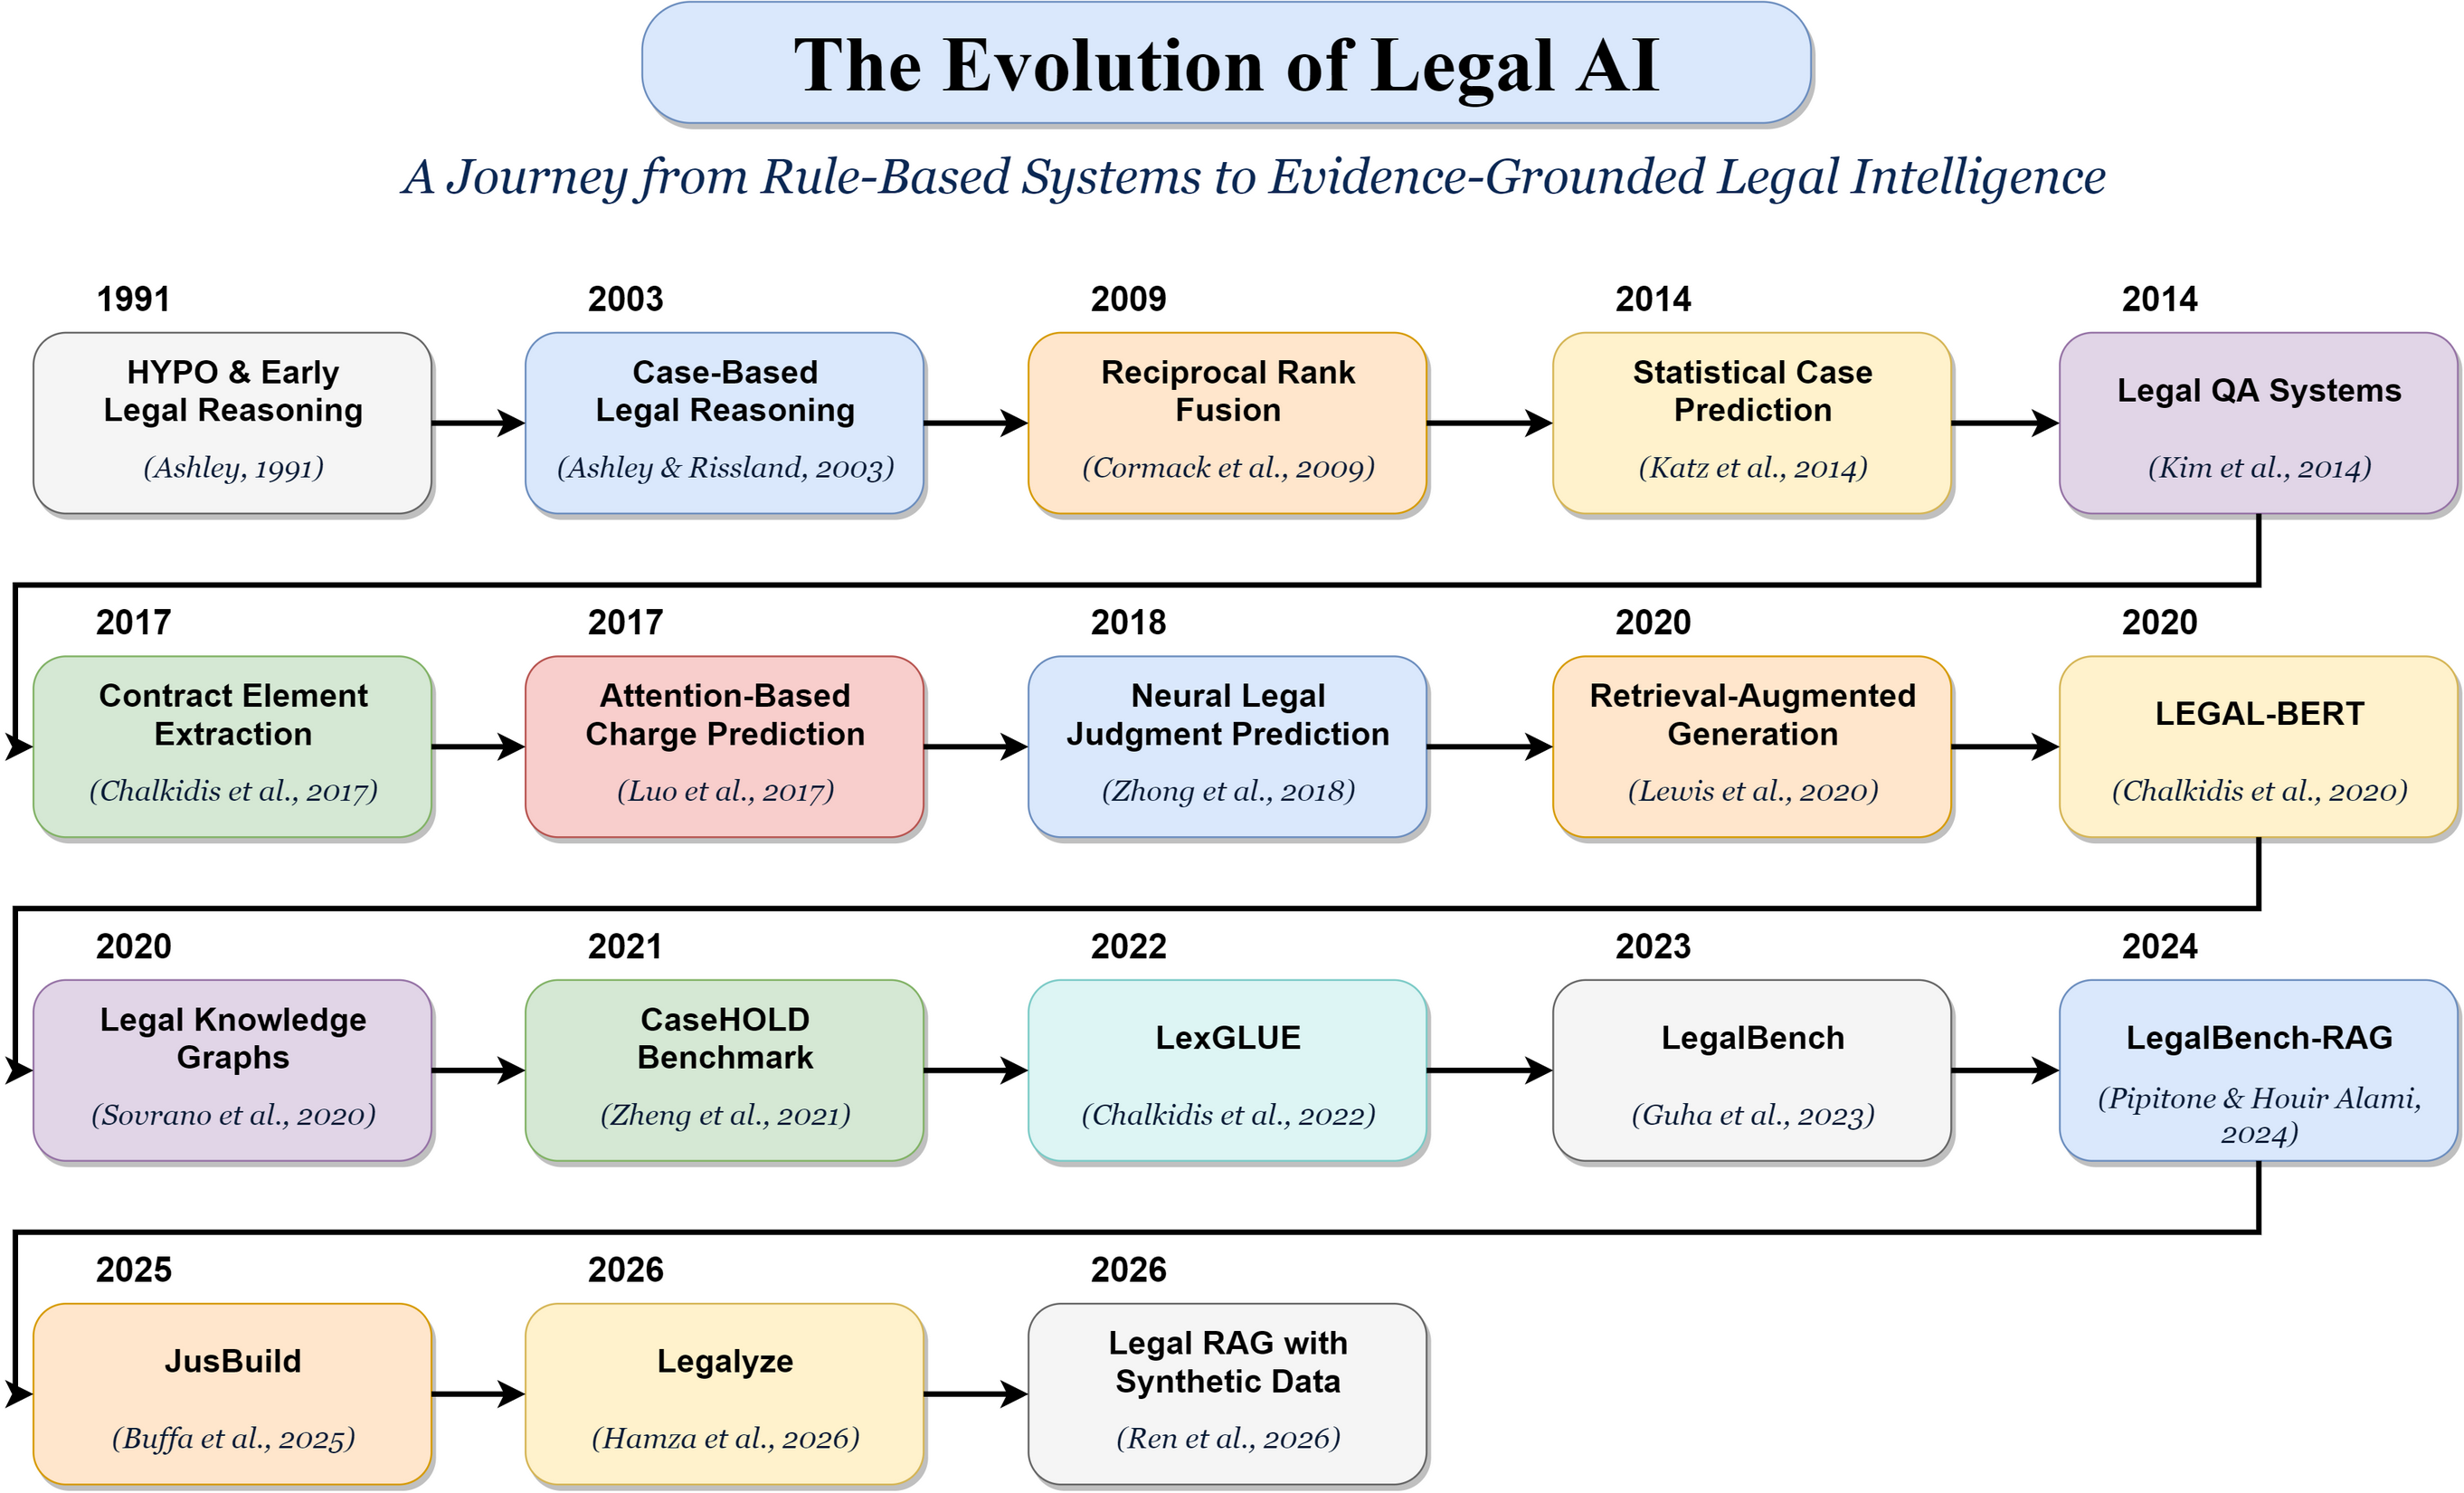
\includegraphics[width=\textwidth]{images/evolution_of_legal_ai.png}
\caption{The evolution of legal AI, 1991--2026, read as a sequence of methodological responses
rather than isolated dates: transparent but non-scaling reasoning systems (case-based reasoning,
rule-based expert systems); learned legal language representations and shared benchmarks; and
recent work on retrieval-augmented generation, reliability, and structure-aware retrieval. The
verified study underpinning each stage is cited, in chronological order, in
Sections~\ref{sec:foundations}--\ref{sec:2026}.}
\label{fig:landscape}
\end{figure*}

\subsection{1991: can a computer reason with cases?}

The field's starting question was foundational: can a computer represent the knowledge and
reasoning that legal professionals use to resolve disputes? Kevin Ashley's HYPO system, published in
1991, gave the first influential answer. HYPO compared a new fact pattern with earlier cases, picked
out the similarities and differences that matter legally, and built arguments from those comparisons
\citep{ashley1991}. This was a deliberate design choice: HYPO did not treat a past decision as a
ready-made answer to a new question, but instead made the comparison process itself part of the
computational problem. The system showed that legal relevance depends on more than textual
similarity between a query and a precedent; it depends on which facts a court would treat as
decisive.

A related line of work, running at the same time, built rule-based expert systems that represented
legal knowledge directly as explicit rules applied to known facts. This made their reasoning easy to
inspect, since a developer could trace exactly which rule and which condition produced a given
output, but it also made them expensive to maintain: legislation changes, exceptions pile up, and
different authorities apply in different circumstances, so a system's rules have to be updated by
hand to keep pace. Structured knowledge representation, including legal ontologies, offered a
complementary response by defining legal concepts and the relationships between them explicitly.
Much later, this idea matured into the knowledge-graph-based legal retrieval systems we discuss in
Section~\ref{sec:lm2023}.

\subsection{2003: case-based reasoning as a form of learning}

Twelve years after HYPO, Ashley and Rissland gave a more general account of why this style of
reasoning works. In \emph{Law, Learning and Representation}, they framed case-based legal reasoning
as a form of \emph{lazy learning}: a court, on this view, holds off generalizing from past cases
until it knows the facts of the new case, rather than committing in advance to one fixed rule
\citep{ashley2003}. This reframing tied case-based reasoning explicitly to machine learning and to
legal information retrieval, and it also clarified what the foundational period had actually
established: a legal AI system needs both a representation of legal knowledge and a method for
applying that representation to the specific facts of a new dispute. A system may have explicit
rules and still fail to identify which facts matter, or it may retrieve a similar case and still
fail to explain why the differences between it and the new dispute matter. That distinction still
organizes legal AI research today.

Alongside reasoning about cases, this period raised a different but related question: how do you
simply \emph{find} the legal documents relevant to a user's need? Legal information retrieval is not
the same problem as legal reasoning; retrieval ranks potentially relevant material, while reasoning
determines how a reader should interpret and apply that material. Early retrieval work leaned
heavily on lexical evidence, which is useful in law because exact wording, section numbers, and
established legal phrases can be decisive, but it can miss material when a query and an
authoritative document describe the same legal concept in different words.

\subsection{2009: a general retrieval technique, outside the legal domain, that the field would later adopt}

The last foundational building block in this period did not come from legal AI at all. In 2009,
\citet{cormack2009} introduced Reciprocal Rank Fusion (RRF) at a general information-retrieval
venue, offering a simple way to combine several ranked lists of search results into one. RRF scores
a candidate document using the reciprocal of its rank in each contributing list,
\begin{equation}
\operatorname{RRF}(d)=\sum_{r \in R}\frac{1}{k+\operatorname{rank}_{r}(d)},
\end{equation}
where $d$ is a candidate document, $R$ is the set of ranked retrieval results under combination,
$\operatorname{rank}_r(d)$ is the rank of $d$ in list $r$, and $k$ is a smoothing constant. Its
appeal is that it combines rankings without needing the underlying retrieval methods to produce
directly comparable scores, which matters because two different retrieval methods often produce
scores on entirely different scales: one method might rely on exact wording, while another might
rely on semantic similarity. We introduce RRF here, at its true publication date, precisely because
it is general purpose; it carries no legal content of its own, and this survey will not pretend
otherwise. It resurfaces more than a decade later, in Section~\ref{sec:rag2024}, once legal retrieval
systems need to combine lexical and semantic evidence, and that is where its legal relevance
actually begins.

\subsection{What this period established}

By the end of this period, legal AI had built up complementary foundations rather than a single
architecture. Case-based reasoning showed that legal relevance requires comparing the facts of
disputes, not just their words. Rule-based systems and legal ontologies showed that legal AI could
represent legal knowledge explicitly, at the cost of ongoing maintenance as the law changes. Early
information retrieval showed that finding candidate legal material is a distinct problem from
reasoning about it. And outside the field entirely, general-purpose information retrieval was
developing techniques, such as rank fusion, that legal AI would not need until its own retrieval
systems grew more sophisticated. None of these approaches alone solved the full challenge of finding
authoritative evidence, keeping its context, and producing a reliable answer. The next advance in
the field's actual chronology did not arrive until 2014, when researchers began asking a different
question: not how should a system reason about a case, but could data alone predict a case's
outcome?
